\section{Design}
I dette projekt er der valgt så vidt muligt at designe alle løsninger med diskret elektronik. Derfor er det valgt at forforstærkeren bygges af common-emitter-trin med uafkoblet emittermodstand. Et common-emitter-trins typiske opbygning er vist på figur \ref{fig:cekobling}.

\begin{figure}[h]
\centering
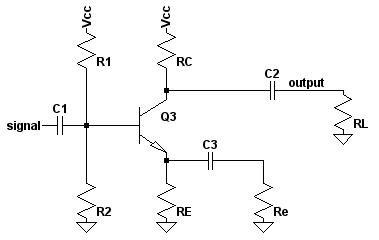
\includegraphics[scale=.6]{teknisk/forforstaerker/ceopkobling.png}
\caption{Generel form på commonemitterkobling med uafkoblet emittermodstand}
\label{fig:cekobling}
\end{figure}


Argumentet for dette valg er, at det er det eneste trin, blandt common-emitter, -base og -collector, hvis spændingsforstærkning er betydeligt over én og ikke, under korrekte omstændigheder, afhænger af transistorparametre. Da transistorparametre blandt andet er afhængige af den anvendte transistors temperatur er det en betragtelig styrke ikke at skulle tage højde for dem. Spændingsforstærkningen i common-emitter-trinnet er dog kun uafhængig af transistorparametre så længe følgende er gældende: $r_o >>R_C \| R_L$, $gm \cdot R_E||R_e$ og $i_e \approx i_c$.
Dette skyldes at forstærkningen er givet ved ligning (\ref{eq:gmbevis}) \cite{ael-mm6}.

\begin{equation}
A_v =  \frac{-gm \cdot R'_L}{1+g_m \cdot R'_e} \approx  -\frac{R'_L}{R'_e} \Biggr\vert _{\frac{1}{g_m}<<R'_e}
\label{eq:gmbevis}
\end{equation}

Hvor $R'_e = R_e || R_E$ og $R'_L = R_L||R_C$. Det vil sige at jo tættere $R_e$ kommer på $\frac{1}{g_m}$ jo mere indflydelse vil denne have på forstærkningen. Disse antagelser vil derfor være gældende gennem hele designet af forforstærkeren. 

Det er valgt at fordele forstærkningen på to trin, da det dermed er muligt at forøge mængden af tilbagekobling, hvilket nedsætter mængden af THD. Da der i dette projekt først designes ud fra maksimal forstærkning uden $R_e$, hvorefter den ønskede forstærkning opnås ved at tilbagekoble det overskydende gennem $R_e$, vil mængden af tilbagekobling være mindre i ét trin med 69,7 ganges forstærkning end i to med den samme samlede forstærkning.
Det første trin vælges til at have en forstærkning på 10 gange og det andet på 6,97 for at opnå den ønskede forstærkning, som vist på figur \ref{blok_forforstaerker}. Grunden til rækkefølgen af trinnene er for ikke at have størst signaludsving og den største forstærkning i samme trin. Dette skyldes at der i en forstærker altid vil være forvrængning og støj. Hvis den største forstærkning kommer sidst, vil denne forvrængning blive forstærket yderligere, hvilket ikke er ønskværdigt. Hvis den største forstærkning derimod kommer først, vil der blive mindst muligt forvrængning med i det endelige signal.

\begin{figure}[h]
\centering
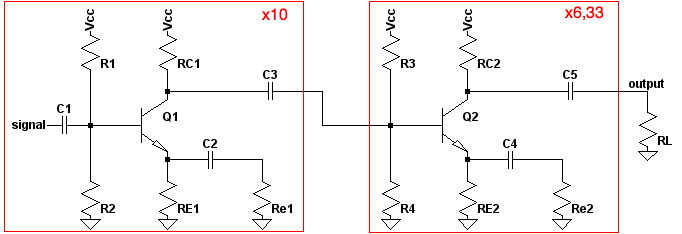
\includegraphics[scale=.6]{teknisk/forforstaerker/blok_forforstaerker.png}
\caption{Blokdiagram over forforstærkerens byggeblokke samt lydsignalets vej}
\label{blok_forforstaerker}
\end{figure}



\subsection*{Design af første trin}
Begge trin designes efter maksimal forstærkning uden $R_e$. Denne forstærkning er givet ved ligning (\ref{eq:dcgain}).

\begin{equation}
|A_{\mathrm{vs}}|=\frac{1}{\left(\frac{V_T \cdot R_C}{V_{R_C}}+\frac{R'_S}{\beta}\right) \left(\frac{1}{R_C}+\frac{1}{R_L}\right)}
\label{eq:dcgain}
\end{equation}
Hvor $R'_S = R_S||R_1||R_2$ og $V_T = 26~\mathrm{mV}$.

For at designe et kredsløb med maksimal forstærkning justeres størrelsen af $R_C$ uden at variere spændingen over den, $V_{R_C}$. Den maksimale $R_C$ findes ved ligning (\ref{eq:rcmaks}).

\begin{equation}
R_{\mathrm{C,maks}} = \sqrt{\frac{R'_S \cdot R_L \cdot V_{R_C}}{\beta \cdot V_T}}
\label{eq:rcmaks}
\end{equation}

I ligning (\ref{eq:rcmaks}) er $R'_S$ defineret som $R_1||R_2||R_S$. Modstanden $R_S$ er fastlagt til 2,2 k\ohm, hvilket er mikrofonens udgangsimpedans \cite{mic-datablad}. Parallelforbindelsen mellem $R_1$ og $R_2$ kan ikke beregnes men skal vælges. Indgangsimpedansen i kredsløbet, som netop er $R_1||R_2$, skal som hovedregel være meget større end udgangsimpedansen i den kreds den belaster. Belastningen, $R_L$, for det første trin bliver indgangsimpedansen i det andet. Indgangsimpedansen i det andet trin bliver $R_3||R_4$ og kan heller ikke beregnes. Da $R_C$ i det første trin ikke kendes endnu vælges indgangsimpedansen i det andet til at være den samme som i det første, altså 22 k\ohm. 
Spændingen $V_{R_C}$ er defineret som værende $V_{CC} - V_{\mathrm{CE,sat}} - V_{R_E} - V_{\mathrm{o,peak}}$, hvor $V_{CC}$ vælges til 15 V så der sikres at der er plads til det ønskede spændingsudsving, $V_{R_E}$ vælges til 3 V og $V_{\mathrm{CE,sat}}$ aflæses i databladet for BC547B  til 0,2 V ved en collectorstrøm på 1 mA \cite{bc547b-datablad}. Der antages at collectorstrømmen cirka bliver 1 mA. Ligeledes aflæses $\beta$ til 250 ved 1 mA i databladet. Spændingen $V_{\mathrm{o,peak}}$ er peakspændingen på udgangen. Dermed bliver peakspændingen en faktor 10 højere end mikrofonens peakspænding på udgangen. Spændingen $V_{\mathrm{o,peak}}$ bliver derfor 316 mV. Modstanden $R_{C1}$ beregnes hermed i ligning (\ref{eq:rcforsteberegning}).

\begin{equation}
R_{\mathrm{C1}} = \sqrt{\frac{22~\mathrm{k}\ohm || 2,2~\mathrm{k}\ohm \cdot (15~\mathrm{V} - 0,2~\mathrm{V} - 3~\mathrm{V} - 0,287~\mathrm{V})}{250 \cdot 26 \cdot 10^{-3}~\mathrm{mV}}}=8,83~\mathrm{k}\ohm
\label{eq:rcforsteberegning}
\end{equation}

Modstanden $R_{\mathrm{E1}}$ bestemmes i ligning (\ref{eq:beregningre1}) under antagelse at $i_e = i_c$.  Strømmen $i_c$ beregnes i ligning(\ref{eq:ff:ic}).

\begin{equation}
\label{eq:ff:ic}
i_C=\frac{V_{R_C}}{R_C}=\frac{11,5~\mathrm{V}}{9,25~\mathrm{k}\ohm}=106,4~\mathrm{mA}
\end{equation}
\begin{equation}
R_{\mathrm{E1}}=\frac{V_{R_{E1}}}{\frac{V_{R_{C1}}}{R_{C1}}}  \Rightarrow R_{\mathrm{E1}}=\frac{3~\mathrm{V}}{106,4~\mathrm{mA}}=2,30~\mathrm{k}\ohm
\label{eq:beregningre1}
\end{equation}


Dernæst beregnes $R_{\mathrm{e1}}$ ud fra hvad den ønskede forstærkning skal være. Ligning (\ref{eq:gmbevis}) benyttes til at beregne $R_{\mathrm{e1}}$ i ligning (\ref{eq:rlilleeberegning}).

\begin{equation}
\label{eq:rlilleeberegning}
A_v = -\frac{R'_L}{R'_e} \Rightarrow  R_{\mathrm{e1}} =-\frac{R_L \cdot R_{\mathrm{C1}} \cdot R_{\mathrm{E1}}}{A_v \cdot R_{\mathrm{E1}} \cdot R_{\mathrm{C1}} + A_v \cdot R_{\mathrm{E1}} \cdot R_L + R_{\mathrm{C1}} \cdot R_L} \Rightarrow R_{\mathrm{e1}} = 868~\ohm
\end{equation}

Biasnetværket, bestående af $R_1$ og $R_2$ beregnes ud fra den spænding, som er påkrævet på basen for at transistoren fungerer som ønsket. Spændingen over base-emitter, $V_{\mathrm{BE}}$, er i databladet aflæst til 0,6 V. Da potentialet på emitteren er 3 V skal potentialet på basen være 3,6 V. Modstandene $R_1$ og $R_2$ kan beregnes ud fra at $V_{R_2}$ skal være 3,6 V og parallelkoblingen $R_1||R_2$ skal være 22 k\ohm. Beregningen udføres i ligning (\ref{eq:r1r21}) og (\ref{eq:r1r22}).

\begin{equation}
\mathrm{3,6~mV} = \mathrm{15~V} \cdot \frac{R_2}{R_1+R_2} 
\label{eq:r1r21}
\end{equation}
\begin{equation}
22~\mathrm{k\ohm} = \frac{R_1 \cdot R_2}{R_1 + R_2}
\label{eq:r1r22}
\end{equation}
De kendte værdier indsættes og de to ligninger med to ubekendte løses. Resultatet er vist i ligning (\ref{eq:r1r2result}).
\begin{equation}
R_1 = 91,7~\mathrm{k}\ohm ~ \wedge ~ R_2=28,9~\mathrm{k}\ohm
\label{eq:r1r2result}
\end{equation}

For at opnå den ønskede frekvensgang skal $C_1$, $C_2$ og $C_3$ dimensioneres således, at den knækfrekvens de hver især frembringer ikke kommer til at forstyrre et ønskede frekvensområde. Da knækfrekvensen er det punkt hvor kurven er faldet 3 dB og frekvensgangen skal, jævnfør kravspecifikationen, være 20 Hz til 20 kHz, er det nødvendigt at knækfrekvens  ligger før 20 Hz. Det vurderes at knækfrekvensen beregnes til at ligge i 2 Hz for at knækfrekvensen ikke giver anledning til en dæmpning af signalet på mere end de tilladte 3 dB. Kondensatorværdierne beregnes med formel (\ref{eq:kondensatorknaek}).

\begin{equation}
C=\frac{1}{\omega \cdot R}=\frac{1}{2\cdot \pi \cdot f \cdot R}
\label{eq:kondensatorknaek}
\end{equation}

I ligning \ref{eq:kondensatorknaek} er $C$ kondensatorens kapacitet og $R$ er den impedans kondensatoren ser ind i. $C_1$ ser ind i forspændingskoblingen i det første forstærkertrin, altså 22 k\ohm. Kondensator $C_2$ ser ind i den AC-koblede emittermodstand, $Re1$, og $C_3$ ser ind i forspændingsnetværket i det andet forstærkertrin, altså 22 k\ohm. Dermed bliver kondensatorernes værdier som følger.

\begin{equation}
C_1=3,58~\mathrm{\my F}~\wedge ~C_2=91,9~\mathrm{\my F}~\wedge ~C_3=3,58~\mathrm{\my F}
\end{equation}



\subsection*{Design af andet trin}
Beregning af andet trin følger samme designprocedure som første trin. Kredsløbet til andet trin er vist på figur \ref{fig:andettrinkreds}.

\begin{figure}[h]
\centering
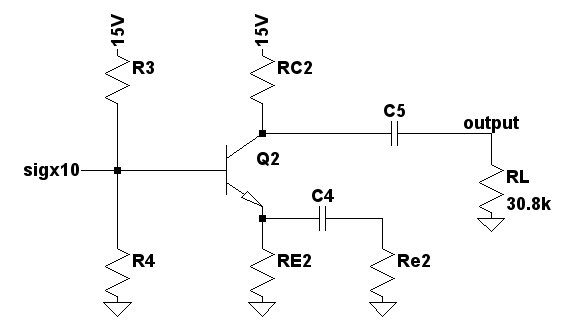
\includegraphics[scale=.6]{teknisk/forforstaerker/andettrinkreds.png}
\caption{Det andet trins kredsløb}
\label{fig:andettrinkreds}
\end{figure}

Det andet trin skal forstærke et signal med en maksimal peakspænding på 287 mV op til 2 V, altså 6,97 gange. Belastningsmodstanden for dette forstærkertrin er bestemt af indgangsvælgeren, som er det næste trin efter forforstærkeren. Indgangsvælgerens indgangsimpedans er 30,8 k\ohm~som beregnet i ligning (\ref{eq:indgangrindgang}). Modstanden $R_S$ er i dette trin givet ved udgangsmodstanden for det første forstærkertrin, som er lig med $R_{\mathrm{C_1}}$, hvilket gør at $R'_S = R_{\mathrm{C_1}} || R_3 || R_4$ kan opstilles. Den maksimale $R_{\mathrm{C_2}}$ beregnes i ligning (\ref{eq:rc2maks}).

\begin{equation}
R_{\mathrm{C_2}} = \sqrt{\frac{R'_S \cdot R_L \cdot V_{R_\mathrm{C_2}}}{\beta \cdot V_T}} = 17,1~\mathrm{k}\ohm
\label{eq:rc2maks}
\end{equation}

Beregningerne af $R_{\mathrm{E2}}$ og $R_{\mathrm{e2}}$ samt kondensatorerne er meget ens med dem for det første forstærkertrin. Derfor er det valgt ikke at vise beregningerne i rapporten. Modstandene $R_3$ og $R_2$ antager samme værdier som henholdsvis $R_1$ og $R_2$, da begge trin skal have samme indgangsimpedans. De beregnede værdier er vist i ligning (\ref{eq:valuestrin2}).

\begin{equation}
R_{E2}=5,24~\mathrm{k\ohm} ~ \wedge ~R_{e2}=2,6~\mathrm{k\ohm} ~ \wedge ~ C_4=30,6~\mathrm{\my F} ~ \wedge ~ C_5=2,6~\mathrm{\my F}
\label{eq:valuestrin2}
\end{equation}

Det endelige kredsløb er vist på figur \ref{fig:forforstaerkersimuleringkredslob} i simuleringsafsnittet.

\subsection*{Simulering}

For at verificere at kredsløbet fungerer som ønsket simuleres det i LTspice. De karakteristika som skal verificeres er spændingsforstærkningen, amplitudekarakteristikken samt harmonisk forvrængning. Kredsløbet der simuleres er vist på figur \ref{fig:forforstaerkersimuleringkredslob}. 

\begin{figure}[h]
\centering
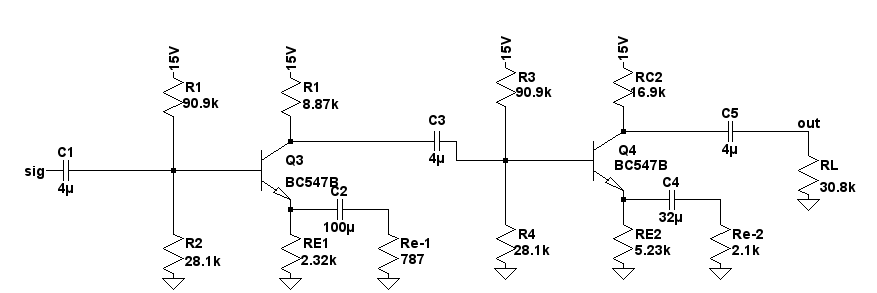
\includegraphics[width=\textwidth]{teknisk/forforstaerker/forforstaerkerendeligkreds.png}
\caption{Forforstærkerens kredsløb med de værdier som vil blive implementeret}
\label{fig:forforstaerkersimuleringkredslob}
\end{figure}

Spændingsforstærkningen af hele trinnet skal være 69,7 gange svarende til 36,9 dB. Forstærkningen vises på figur \ref{fig:amplitude-forforstaerker} ved hjælp af en amplitudekarakteristik, således at spændet fra 20 Hz til 20 kHz tydeligt kan ses. 


\begin{figure}[h]
\centering
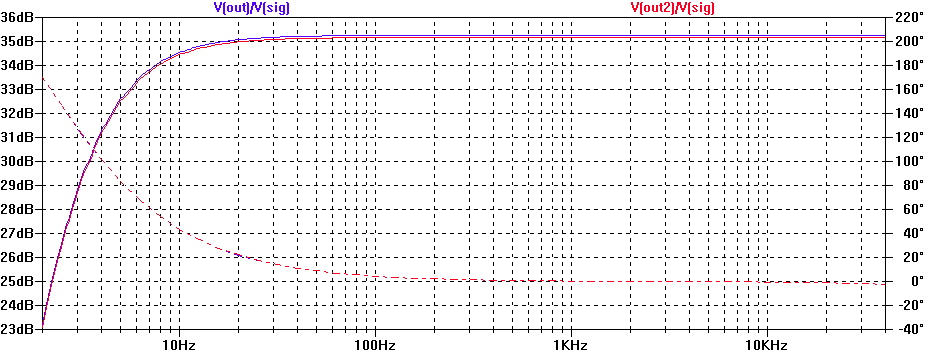
\includegraphics[width=\textwidth]{teknisk/forforstaerker/amplitudeforforstaerker.png}
\caption{Forforstærkerens amplitude karakteristik med modstandsværdier fra figur \ref{fig:forforstaerkersimuleringkredslob}}
\label{fig:amplitude-forforstaerker}
\end{figure}

Simuleringen viser at forstærkningen ved 1 kHz, som er referencen jævnfør kravspecifikationen, er 35 dB hvor den skulle have være 36,9 dB. Dermed må det konkluderes at beregningen af forforstærkertrinnene indeholder usikkerheder. Usikkerhederne vurderes til at bestå i de antagelser som defineres før beregningerne: 
\[ r_o >>R_C || R_L \]
\[ g_m \cdot R_E||R_e\]
\[i_e \approx i_c\]
For at have en simulering der kan sammenlignes med de målte data er det valgt at korrigere forstærkningen i trinnene. Dette gøres ifølge ligning (\ref{eq:gmbevis}) ved justeres på den AC-koblede emittermodstand, $R_{e1}$ og $R_{e2}$. I ligning (\ref{eq:nyerevalues}) er de nye værdier for disse modstande anvist. Modstandsværdierne er fundet ved først at justere $R_{e1}$ til det første trin giver den korrekte forstærkning for derefter at gøre det samme med det andet trin.

\begin{equation}
R_{e1}=790~\ohm~\wedge ~R_{e2}=2,1~\mathrm{k}\ohm
\label{eq:nyerevalues}
\end{equation}

Med de nye modstandsværdier bliver amplituden som vist på figur \ref{fig:rigtigamplitudeforforstaerker}.

\begin{figure}[h]
\centering
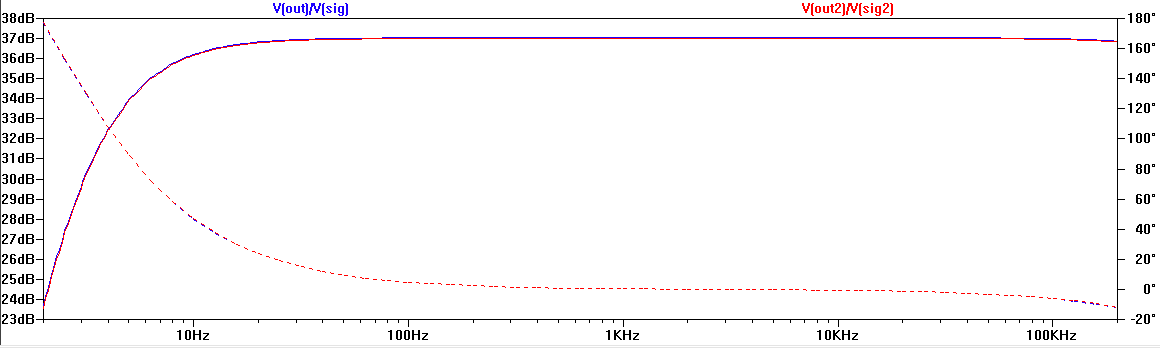
\includegraphics[width=\textwidth]{teknisk/forforstaerker/rigtigamplitude.png}
\caption{Forforstærkerens amplitudekarakteristik efter korrektion af forstærkning}
\label{fig:rigtigamplitudeforforstaerker}
\end{figure}

På figur \ref{fig:rigtigamplitudeforforstaerker} ses det at forstærkningen nu er korrigeret. Derudover fremgår det at dæmpningen fra 20 kHz til 20 Hz er 0,2 dB. Dermed overholdes kravet om at dæmpningen i dette område, som skal være under 0,375 dB. 

Den harmoniske forvrængning skal ifølge kravspecifikationen være under 0,5 \%. Ifølge LTspice er den harmoniske forvrængning, ved 1 kHz og maksimal peakspænding på indgangen, 0,2 \%. Forvrængningsmålingen er udført ved maksimal peakspænding, da forvrængningen i trinnet vil være højest ved denne situation. 